% Build: cd paper && tectonic main.tex   (figures and numbers: python paper/make_figures.py from the repo root)
\documentclass[10pt,twocolumn,letterpaper]{article}
\usepackage[margin=0.75in,columnsep=0.25in]{geometry}
\usepackage[T1]{fontenc}
\usepackage{newtxtext,newtxmath}
\usepackage{microtype,graphicx,booktabs,xcolor,amsmath,siunitx,caption,subcaption}
\usepackage[hidelinks]{hyperref}
\usepackage{pgfplots}
\pgfplotsset{compat=1.18}
\usepgfplotslibrary{groupplots}
\usetikzlibrary{positioning,arrows.meta,calc,fit,backgrounds}
\captionsetup{font=small,labelfont=bf}
\captionsetup[sub]{font=footnotesize}

% generated by paper/make_figures.py
\newcommand{\ADemos}{187}
\newcommand{\AId}{26.7}
\newcommand{\AIdK}{8/30}
\newcommand{\AIdMovedK}{10/30}
\newcommand{\AInBox}{36}
\newcommand{\AOod}{20}
\newcommand{\AOodK}{4/20}
\newcommand{\AOodMovedK}{10/20}
\newcommand{\BDemos}{177}
\newcommand{\BId}{63.3}
\newcommand{\BIdK}{19/30}
\newcommand{\BIdMovedK}{24/30}
\newcommand{\BInBox}{51}
\newcommand{\BOod}{40}
\newcommand{\BOodK}{8/20}
\newcommand{\BOodMovedK}{11/20}
\newcommand{\CDemos}{287}
\newcommand{\CId}{56.7}
\newcommand{\CIdK}{17/30}
\newcommand{\CIdMovedK}{29/30}
\newcommand{\CInBox}{136}
\newcommand{\COod}{50}
\newcommand{\COodK}{10/20}
\newcommand{\COodMovedK}{15/20}
\newcommand{\CollNoise}{83/120}
\newcommand{\CollV}{100/106}
\newcommand{\CollWideA}{94/100}
\newcommand{\CollWideB}{93/100}
\newcommand{\DDemos}{277}
\newcommand{\DId}{66.7}
\newcommand{\DIdK}{20/30}
\newcommand{\DIdMovedK}{23/30}
\newcommand{\DInBox}{151}
\newcommand{\DOod}{15}
\newcommand{\DOodK}{3/20}
\newcommand{\DOodMovedK}{8/20}
\newcommand{\DensityRatio}{2.8}
\newcommand{\ExpertId}{100}
\newcommand{\ExpertIdK}{30/30}
\newcommand{\ExpertIdMovedK}{30/30}
\newcommand{\ExpertOod}{90}
\newcommand{\ExpertOodK}{18/20}
\newcommand{\ExpertOodMovedK}{19/20}
\newcommand{\ExpertTimedId}{96.7}
\newcommand{\ExpertTimedIdK}{29/30}
\newcommand{\ExpertTimedIdMovedK}{30/30}
\newcommand{\ExpertTimedOod}{85}
\newcommand{\ExpertTimedOodK}{17/20}
\newcommand{\ExpertTimedOodMovedK}{19/20}
\newcommand{\OodX}{6}
\newcommand{\OodYaw}{20}
\newcommand{\PinchPose}{x = -0.9\,cm, y = -1.0\,cm, yaw = -2.2$^\circ$}
\newcommand{\PmixId}{= .02}
\newcommand{\PmixNoiseId}{= .58}
\newcommand{\PmixNoiseOod}{= .09}
\newcommand{\PmixOod}{= .55}
\newcommand{\PwideId}{< .001}
\newcommand{\PwideNoiseId}{= .03}
\newcommand{\PwideNoiseOod}{= .29}
\newcommand{\SettleLen}{522}
\newcommand{\TimedDemos}{100}
\newcommand{\TimedId}{0}
\newcommand{\TimedIdK}{0/30}
\newcommand{\TimedIdMovedK}{0/30}
\newcommand{\TimedIdleMax}{45}
\newcommand{\TimedIdleMedian}{23}
\newcommand{\TimedIdlePct}{30}
\newcommand{\TimedIdleRuns}{8.2}
\newcommand{\TimedInBox}{100}
\newcommand{\TimedLen}{714}
\newcommand{\TimedOod}{0}
\newcommand{\TimedOodK}{0/20}
\newcommand{\TimedOodMovedK}{0/20}
\newcommand{\TracePose}{x = +1.1\,cm, y = -1.8\,cm, yaw = -9.2$^\circ$}
\newcommand{\TraceSettleTicks}{524}
\newcommand{\TraceTimedTicks}{714}
\newcommand{\TrainX}{4}
\newcommand{\TrainYaw}{10}
\newcommand{\VtwoDemos}{100}
\newcommand{\VtwoId}{86.7}
\newcommand{\VtwoIdK}{26/30}
\newcommand{\VtwoIdMovedK}{28/30}
\newcommand{\VtwoInBox}{100}
\newcommand{\VtwoOod}{35}
\newcommand{\VtwoOodK}{7/20}
\newcommand{\VtwoOodMovedK}{10/20}
\newcommand{\WideVolume}{4.5}


% chart roles (validated categorical slots 1 and 2; text never wears series colour)
\definecolor{sone}{HTML}{2A78D6}
\definecolor{stwo}{HTML}{EB6834}
\definecolor{ink}{HTML}{0B0B0B}
\definecolor{inktwo}{HTML}{52514E}
\definecolor{inkthree}{HTML}{8A8983}
\definecolor{rule}{HTML}{E2E1DC}
\definecolor{idlefill}{HTML}{D9D8D2}
\definecolor{boxfill}{HTML}{F4F3EF}

\pgfplotsset{
  base/.style={
    axis line style={inkthree}, tick style={inkthree}, major tick length=2pt,
    tick label style={font=\scriptsize, text=inktwo}, label style={font=\scriptsize, text=inktwo},
    title style={font=\scriptsize\bfseries, text=ink, yshift=-1ex},
    grid=major, major grid style={rule, line width=.3pt},
    legend style={font=\scriptsize, draw=none, fill=none, text=inktwo},
    legend cell align=left, axis lines=left, enlargelimits=false},
  posemap/.style={base, scale only axis, width=3.1cm, height=3.1cm,
    xmin=-6.6, xmax=6.6, ymin=-6.6, ymax=6.6, xtick={-4,0,4}, ytick={-4,0,4}, axis lines=box},
}
\tikzset{
  trainbox/.style={inktwo, dashed, line width=.5pt},
  oodbox/.style={inkthree, line width=.5pt},
  idle/.style={fill=idlefill},
  grip/.style={stwo, line width=.7pt, densely dashed},
  stage/.style={draw=inkthree, rounded corners=2pt, fill=boxfill, align=center, font=\scriptsize, inner sep=3pt, text=ink},
  flow/.style={-{Stealth[length=4pt]}, inktwo, line width=.6pt},
}

\newcommand{\ttt}[1]{\texttt{\small #1}}
\newcommand{\tts}[1]{\texttt{\scriptsize #1}}

\title{\Large Pose-Randomized Demonstrations and an ACT Baseline\\for Bimanual Detent-Latch Bottle Opening}
\author{Monish Soundar Raj\\[2pt]
\small COMP 790 final project, policy-learning part. Team: Jr-Jen Chen, Akil Dickerson, Ye Mon, Monish Soundar Raj.\\
\small Code: \url{https://github.com/jjenchen-unc/detent-bottle-sim} (\ttt{bench/}, pull request \#1)}
\date{}

\begin{document}
\maketitle

\begin{abstract}
The detent-bottle task asks two Franka Panda arms in MuJoCo to hold a bottle, fold a small safety loop past a
detent, and press a rocker button that springs the lid open. We turn the task into a benchmark for learned
policies. We randomize the bottle pose, record scripted demonstrations in the Gym interface, and evaluate every
policy on fixed held-out poses inside (\ttt{test\_id}) and outside (\ttt{test\_ood}) the training range. Along
the way we found that ACT could not learn from the reference opener's demonstrations. The arm reaches each
target early and then sits still until a timer expires, so the moment to close the gripper is not visible in the
observation. An ACT policy trained on them scored \TimedId\% even though it followed the expert to within a few
millimetres. Ending each segment once the robot comes to rest raised the same ACT to \VtwoId\% on
\ttt{test\_id} and \VtwoOod\% on \ttt{test\_ood}, using only cameras and joint readings. We then tested two
ideas for positions outside the training range: a wider training range and DART-style noise injection. With a
fixed budget of about 200 demonstrations, spreading them over a \WideVolume$\times$ larger pose box cut
\ttt{test\_id} success to \AId\%. Adding wide demonstrations to the original ones gave the best \ttt{test\_ood}
score (\COod\%) but lost precision at the button press. Noise bursts gave no consistent gain once demonstration
density was matched. All results are for ACT with one training seed per configuration.
\end{abstract}

\begin{figure*}[t]
  \centering
  \setlength{\tabcolsep}{1pt}
  \begin{tabular}{@{}cccccc@{}}
    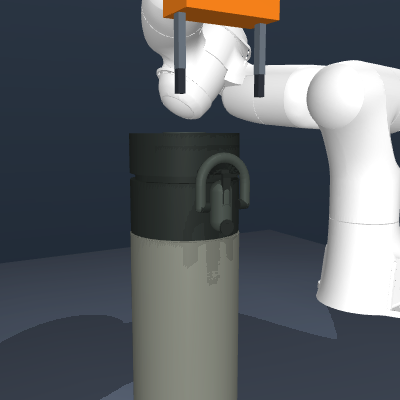
\includegraphics[width=.162\textwidth]{figures/stage_start.png} &
    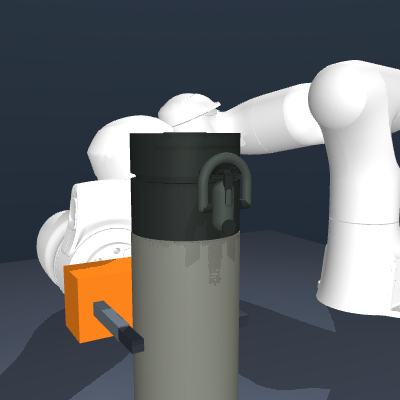
\includegraphics[width=.162\textwidth]{figures/stage_grip.png} &
    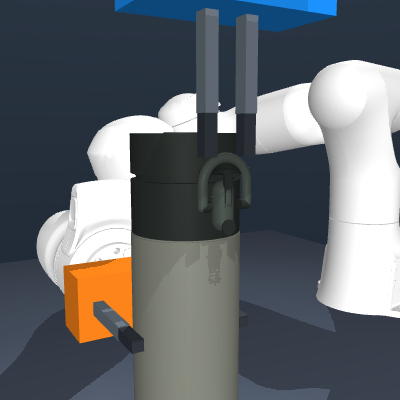
\includegraphics[width=.162\textwidth]{figures/stage_pinch.png} &
    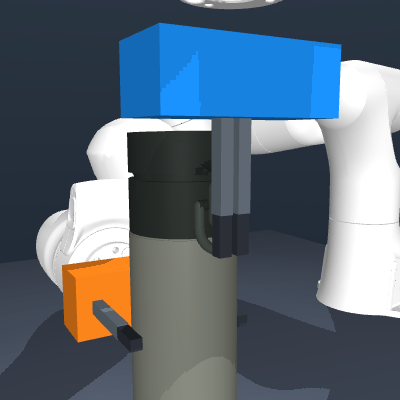
\includegraphics[width=.162\textwidth]{figures/stage_fold.png} &
    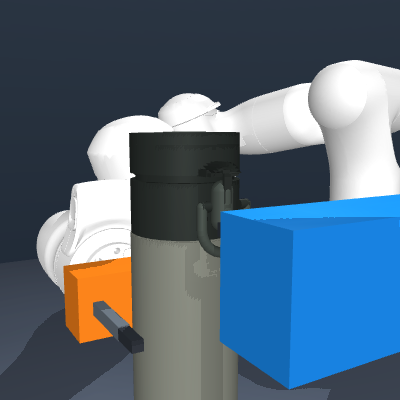
\includegraphics[width=.162\textwidth]{figures/stage_press.png} &
    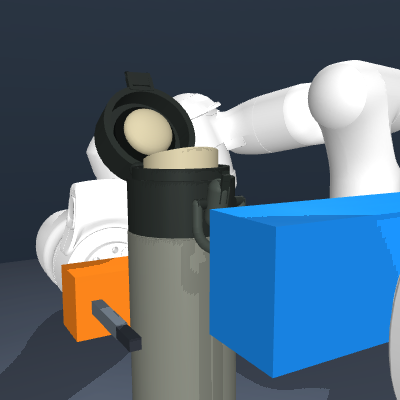
\includegraphics[width=.162\textwidth]{figures/stage_open.png} \\[-1pt]
    \scriptsize start & \scriptsize 1.\ grip the bottle (right) & \scriptsize 2.\ pinch the loop (left) &
    \scriptsize 3.\ fold the loop past the detent & \scriptsize 4.\ reach the rocker button & \scriptsize 5.\ press; lid springs open \\[3pt]
    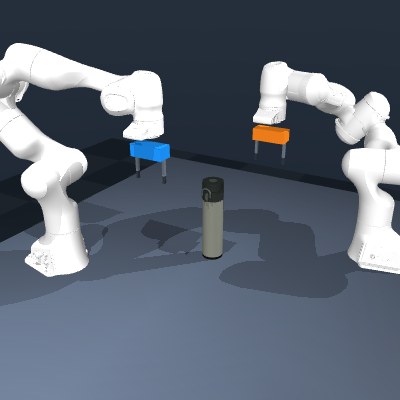
\includegraphics[width=.162\textwidth]{figures/overview.png} &
    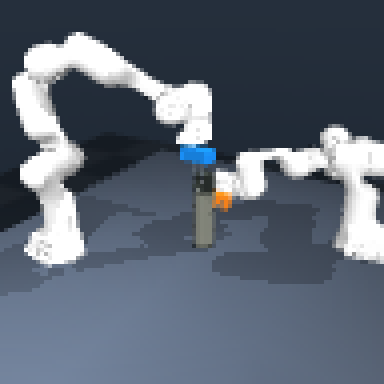
\includegraphics[width=.162\textwidth]{figures/input_agentview.png} &
    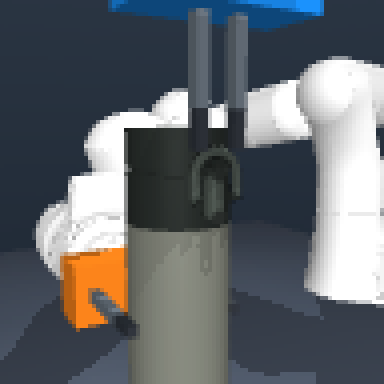
\includegraphics[width=.162\textwidth]{figures/input_frontview.png} &
    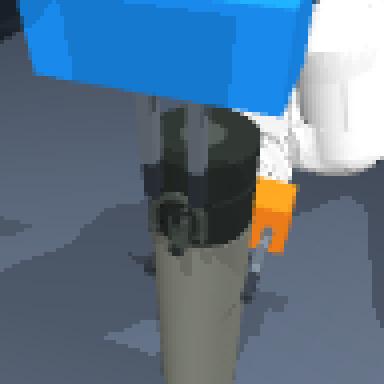
\includegraphics[width=.162\textwidth]{figures/input_topview.png} &
    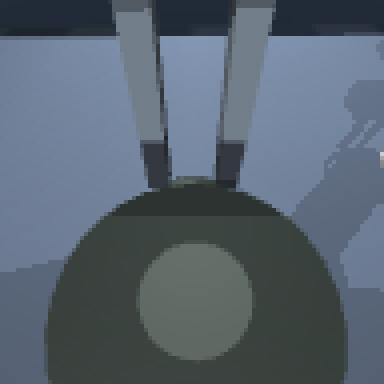
\includegraphics[width=.162\textwidth]{figures/input_left_wrist.png} &
    
\includegraphics[width=.162\textwidth]{figures/input_right_wrist.png} \\[-1pt]
    \scriptsize scene & \scriptsize policy input: agentview & \scriptsize frontview & \scriptsize topview &
    \scriptsize left wrist & \scriptsize right wrist
  \end{tabular}
  \caption{The task. Top: the settle expert at the default bottle pose (front close-up camera). The blue left
  gripper pinches the safety loop, folds it down past the detent and presses the rocker. The orange right
  gripper holds the bottle. Bottom: the full scene, and the five $96\times96$ camera images an ACT policy sees
  (shown during the pinch, upscaled without smoothing).}
  \label{fig:task}
\end{figure*}

\section{Introduction}
The detent-bottle environment (by Jr-Jen Chen) simulates a bottle whose lid is held shut by a detent latch. A
safety loop must be folded down past a detent before a rocker button can release the spring-loaded lid
(Fig.~\ref{fig:task}). The task is long-horizon (about 500 control ticks, five phases) and bimanual, and it
depends on millimetre-scale contact: the loop is a thin wire and the button is small. The environment ships with
a scripted reference opener that works in fixed world coordinates. \ttt{reset()} always produces the same
state. So the repository by itself gives one trajectory, and a policy evaluated at the default pose could simply
memorise it.

This report covers the policy-learning part of the project. Our contributions are:
\begin{itemize}\itemsep0pt
  \item a \textbf{benchmark layer} (\ttt{bench/}). It provides randomized bottle poses, a pose-aware scripted
  expert, demonstration collection in the Gym format, and a shared evaluation harness with fixed in-range and
  out-of-range test poses that any policy can plug into (Sec.~\ref{sec:bench});
  \item a \textbf{likely explanation for why ACT fails on the reference demonstrations} (idle waits that are
  not visible in the observation), and a fix that changes the expert only where it is idle
  (Sec.~\ref{sec:idle});
  \item an \textbf{ACT baseline} that uses cameras and proprioception only and reaches \VtwoId\% on
  \ttt{test\_id} (Sec.~\ref{sec:act});
  \item a \textbf{study of pose coverage and noise injection} for out-of-range poses, with the negative and
  mixed results reported as they came out (Sec.~\ref{sec:results}).
\end{itemize}

\section{Task and environment}\label{sec:env}
The scene has two torque-controlled Franka Panda arms and one free bottle, simulated in MuJoCo~\cite{mujoco}
behind a Gymnasium~\cite{gymnasium} interface (\ttt{DetentBottle-v0}).
\begin{itemize}\itemsep0pt
  \item \textbf{Control and episodes.} The control rate is 20\,Hz (50\,ms ticks) and an episode has at most
  2400 ticks.
  \item \textbf{Actions.} The 14-D action holds, per arm, a translation step (scaled to at most 2\,cm), a
  rotation step (at most 0.1\,rad) and an absolute jaw command. The environment keeps a persistent Cartesian
  target for each tool, and the action moves that target.
  \item \textbf{Observations.} Five RGB cameras (three fixed, two on the wrists) plus joint positions and
  velocities, finger positions, tool poses, wrist force--torque and finger forces.
  \item \textbf{Success.} The lid is open past $60^\circ$ with the bottle upright for 0.4\,s.
\end{itemize}

We made two changes outside the policy code. First, the bottle pose argument documents yaw in degrees, but the
scene compiler read it as radians, so a requested $10^\circ$ rotated the bottle by about $-147^\circ$. We fixed
this and added a test. Second, the environment only counts the bottle as fallen if it leaves the table
($z<0.76$\,m), so a bottle lying on its side runs to the time limit. The evaluation harness therefore ends an
episode as \emph{tipped} once the bottle tilts past $60^\circ$. The environment itself is unchanged.

\section{Benchmark}\label{sec:bench}
\paragraph{Poses and splits.} A pose is an offset $(x, y, \text{yaw})$ of the bottle from its default
placement. Training poses come from a box of $\pm\TrainX$\,cm and $\pm\TrainYaw^\circ$. The held-out
\ttt{test\_id} split has 30 poses from the same box, drawn with a different seed. \ttt{test\_ood} has 20 poses
from the $\pm\OodX$\,cm, $\pm\OodYaw^\circ$ box with at least one coordinate outside the training box
(Fig.~\ref{fig:poses}). For Sec.~\ref{sec:results} we add \ttt{train\_wide}, which samples the whole outer box.
For a policy trained on it, \ttt{test\_ood} is inside the training range. Its \ttt{test\_ood} score then
measures coverage, not out-of-distribution generalisation. A test checks that no training pose appears in either
test split.

\begin{figure}[t]
\centering
\begin{tikzpicture}
\begin{groupplot}[group style={group size=2 by 1, horizontal sep=5mm, yticklabels at=edge left},
  posemap, xlabel={$x$ (cm)}, legend style={at={(.5,-.3)}, anchor=north, legend columns=1}]
\nextgroupplot[title={training demonstrations}, ylabel={$y$ (cm)}]
  \draw[oodbox] (axis cs:-6,-6) rectangle (axis cs:6,6);
  \draw[trainbox] (axis cs:-4,-4) rectangle (axis cs:4,4);
  \addplot[only marks, mark=*, mark size=1.1pt, sone, draw=white, line width=.2pt] table[x=x, y=y] {figures/plotdata/poses_train.dat};
  \addplot[only marks, mark=triangle, mark size=1.5pt, stwo, line width=.5pt] table[x=x, y=y] {figures/plotdata/poses_train_wide.dat};
  \legend{\tts{expert\_v2} (\VtwoDemos), wide clean (\ADemos)}
\nextgroupplot[title={held-out test poses}]
  \draw[oodbox] (axis cs:-6,-6) rectangle (axis cs:6,6);
  \draw[trainbox] (axis cs:-4,-4) rectangle (axis cs:4,4);
  \addplot[only marks, mark=*, mark size=1.4pt, sone, draw=white, line width=.2pt] table[x=x, y=y] {figures/plotdata/poses_test_id.dat};
  \addplot[only marks, mark=square, mark size=1.4pt, stwo, line width=.6pt] table[x=x, y=y] {figures/plotdata/poses_test_ood.dat};
  \legend{\tts{test\_id} (30), \tts{test\_ood} (20)}
\end{groupplot}
\end{tikzpicture}
\caption{Bottle positions (yaw not shown). Dashed square: training box ($\pm4$\,cm, $\pm10^\circ$). Solid
square: wide box ($\pm6$\,cm, $\pm20^\circ$). \ttt{test\_ood} poses have at least one of $x$, $y$ or yaw
outside the training box, so some lie inside the dashed square in $x$--$y$ with a large yaw.}
\label{fig:poses}
\end{figure}

\paragraph{Pose-aware expert.} The reference opener is a sequence of 13 timed segments (tool target, jaw width,
tick count) in five phases. We move every target rigidly into the bottle's frame and drive it through the Gym
action space, so the demonstrations use exactly the interface a learned policy uses. The expert is privileged:
it is told the pose. A one-axis sweep showed that it succeeds for $x, y$ offsets up to $\pm8$\,cm. It fails
for yaw at $-20^\circ$ and beyond, where the loop is never folded, and this caps every \ttt{test\_ood} score.
Only successful episodes are kept (\CollV{} for the first 100 timed demonstrations).

\paragraph{Evaluation.} A policy is a factory \ttt{make\_policy(pose, **kw)} that returns
\ttt{policy(obs, sim)} $\rightarrow$ action. Learned policies must ignore \ttt{pose} and \ttt{sim}. The harness
runs each split in parallel and reports four things: success rate, the rate at which the loop is folded past
the detent ($>150^\circ$), the lid-open rate, and termination reasons. Results from different policies sit side
by side in one table (\ttt{python -m bench.report}). Fig.~\ref{fig:pipeline}a shows the data flow.

\begin{figure*}[t]
\centering
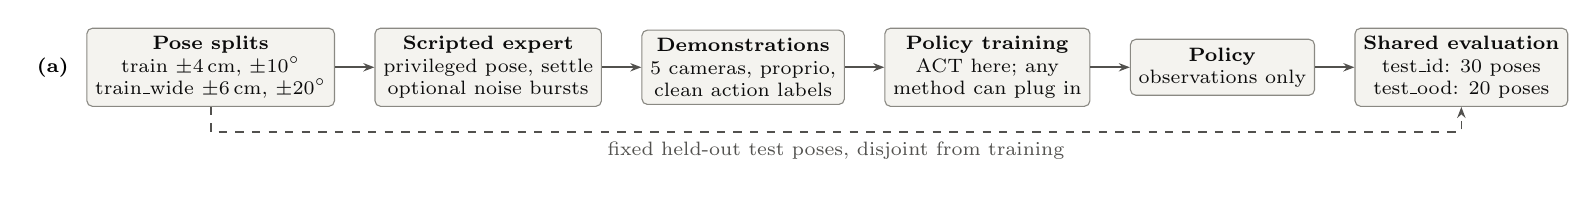
\begin{tikzpicture}[node distance=5mm]
  \node[stage] (poses) {\textbf{Pose splits}\\train $\pm4$\,cm, $\pm10^\circ$\\train\_wide $\pm6$\,cm, $\pm20^\circ$};
  \node[stage, right=of poses] (expert) {\textbf{Scripted expert}\\privileged pose, settle\\optional noise bursts};
  \node[stage, right=of expert] (demos) {\textbf{Demonstrations}\\5 cameras, proprio,\\clean action labels};
  \node[stage, right=of demos] (train) {\textbf{Policy training}\\ACT here; any\\method can plug in};
  \node[stage, right=of train] (policy) {\textbf{Policy}\\observations only};
  \node[stage, right=of policy] (eval) {\textbf{Shared evaluation}\\test\_id: 30 poses\\test\_ood: 20 poses};
  \draw[flow] (poses) -- (expert);
  \draw[flow] (expert) -- (demos);
  \draw[flow] (demos) -- (train);
  \draw[flow] (train) -- (policy);
  \draw[flow] (policy) -- (eval);
  \draw[flow, dashed] (poses.south) -- ++(0,-.32) -| node[pos=.25, below, font=\scriptsize, text=inktwo] {fixed held-out test poses, disjoint from training} (eval.south);
  \node[font=\scriptsize\bfseries, anchor=east] at ($(poses.west)+(-.1,0)$) {(a)};
\end{tikzpicture}

\vspace{6pt}
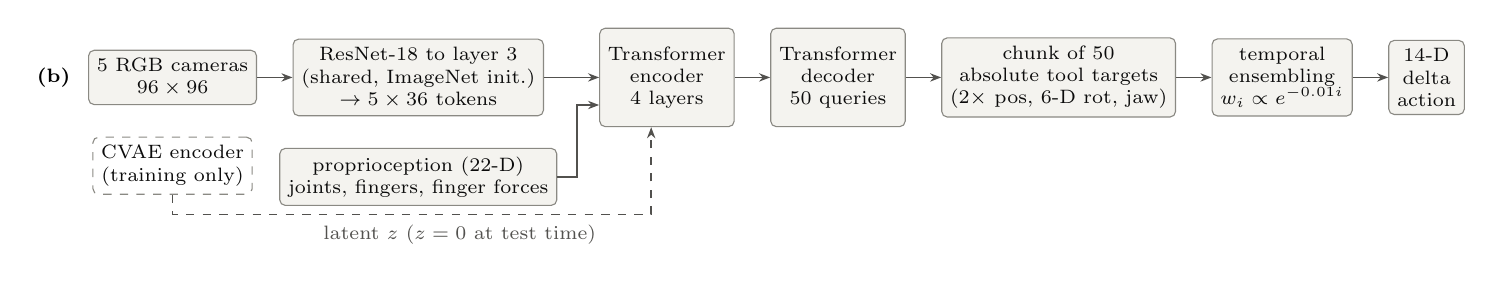
\begin{tikzpicture}[node distance=4.5mm]
  \node[stage] (cams) {5 RGB cameras\\$96\times96$};
  \node[stage, right=of cams] (resnet) {ResNet-18 to layer 3\\(shared, ImageNet init.)\\$\rightarrow 5\times36$ tokens};
  \node[stage, right=7mm of resnet, minimum height=1.25cm] (enc) {Transformer\\encoder\\4 layers};
  \node[stage, right=of enc, minimum height=1.25cm] (dec) {Transformer\\decoder\\50 queries};
  \node[stage, right=of dec] (chunk) {chunk of 50\\absolute tool targets\\($2\times$ pos, 6-D rot, jaw)};
  \node[stage, right=of chunk] (ens) {temporal\\ensembling\\$w_i\propto e^{-0.01 i}$};
  \node[stage, right=of ens] (act) {14-D\\delta\\action};
  \node[stage, below=4mm of resnet] (prop) {proprioception (22-D)\\joints, fingers, finger forces};
  \node[stage, below=4mm of cams, dashed, fill=white] (cvae) {CVAE encoder\\(training only)};
  \draw[flow] (cams) -- (resnet); \draw[flow] (resnet) -- (enc); \draw[flow] (enc) -- (dec);
  \draw[flow] (dec) -- (chunk); \draw[flow] (chunk) -- (ens); \draw[flow] (ens) -- (act);
  \draw[flow] (prop.east) -- ++(.25,0) |- ($(enc.west)+(0,-.35)$);
  \draw[flow, dashed] (cvae.south) -- ++(0,-.25) -| node[pos=.3, below, font=\scriptsize, text=inktwo] {latent $z$ ($z=0$ at test time)} ($(enc.south)+(-.2,0)$);
  \node[font=\scriptsize\bfseries, anchor=east] at ($(cams.west)+(-.1,0)$) {(b)};
\end{tikzpicture}
\caption{(a) The benchmark. Demonstrations and test episodes come from the same pose sampler with disjoint
seeds; every policy is scored on the same held-out poses. (b) The ACT baseline. The model predicts absolute
tool targets, which the policy turns into the environment's delta action by tracking the environment's targets
itself.}
\label{fig:pipeline}
\end{figure*}

\section{Idle waits in the reference demonstrations}\label{sec:idle}
Our first ACT, trained on 100 timed demonstrations, scored \TimedIdK{} on \ttt{test\_id} and \TimedOodK{} on
\ttt{test\_ood}. It brought both hands to within a few millimetres of the grasp points and then never closed
either gripper. Replayed open-loop on held-out demonstrations, its predicted targets at the grip and the
pinch were within 1--3\,mm of the expert's. So it had learned where to go but not when to close. This check
does not rule out every model or deployment problem, but it points at the timing of the gripper commands.

The cause is in the demonstrations (Fig.~\ref{fig:idle}). Each segment of the reference opener lasts a fixed
number of ticks. In most of them the arm reaches its target early and then stays completely still until the
clock runs out, and only then does the gripper close or the next move begin. Over the whole timed dataset,
\TimedIdlePct\% of all ticks belong to such idle stretches of at least 10 ticks. There are \TimedIdleRuns{} of
them per episode, with a median length of \TimedIdleMedian{} ticks and a maximum of \TimedIdleMax. During a
stretch the observation barely changes while the correct action switches from ``wait'' to ``close''. A policy
that sees only the current observation (or a short history) has no visible cue for when the wait is over, and
a loss that averages the two labels favours waiting, which matches what we observed. We tested this with ACT
only. Policies that model multimodal actions, such as diffusion policies~\cite{diffusion_policy}, or that have
longer memory may be affected differently.

The fix changes only the expert's timing. A settle expert (\ttt{--settle}) ends a segment once two conditions
hold for 3 consecutive ticks: both tools are within 1.5\,mm of their targets, and the joints and fingers have
stopped moving ($<10^{-4}$\,rad and $<10^{-5}$\,m per tick). Each segment lasts at least 5 ticks, and the
original tick count remains the upper bound. Contact segments such as the fold still run their full length,
because the arm is pushing against the loop and never comes to rest. Each next move is now triggered by
something visible: the arm has arrived. Episodes shrink from \TimedLen{} to \SettleLen{} ticks on average,
every one of the 100 settle demonstrations succeeded, and the expert itself improved slightly
(Table~\ref{tab:results}). The default (\ttt{settle=False}) still reproduces the original opener action for
action.

\begin{figure}[t]
\centering
\def\ymaxtrace{100}
\begin{tikzpicture}
\begin{groupplot}[group style={group size=1 by 2, vertical sep=7mm, xticklabels at=edge bottom},
  base, width=.96\columnwidth, height=2.9cm, xmin=0, xmax=720, ymin=0, ymax=\ymaxtrace, ytick={0,50,100},
  ylabel={tool speed (mm/s)}, ylabel style={yshift=-1mm}]
\nextgroupplot[title={timed reference opener (\TraceTimedTicks{} ticks)}]
  \fill[idle] (axis cs:56,0) rectangle (axis cs:91,\ymaxtrace);
\fill[idle] (axis cs:138,0) rectangle (axis cs:181,\ymaxtrace);
\fill[idle] (axis cs:239,0) rectangle (axis cs:271,\ymaxtrace);
\fill[idle] (axis cs:280,0) rectangle (axis cs:292,\ymaxtrace);
\fill[idle] (axis cs:351,0) rectangle (axis cs:386,\ymaxtrace);
\fill[idle] (axis cs:573,0) rectangle (axis cs:596,\ymaxtrace);
\fill[idle] (axis cs:652,0) rectangle (axis cs:666,\ymaxtrace);
\fill[idle] (axis cs:688,0) rectangle (axis cs:701,\ymaxtrace);
\draw[grip] (axis cs:295,0) -- (axis cs:295,\ymaxtrace);
\draw[grip] (axis cs:410,0) -- (axis cs:410,\ymaxtrace);
\draw[grip] (axis cs:595,0) -- (axis cs:595,\ymaxtrace);

  \addplot[sone, line width=.7pt, mark=none] table[x=t, y=speed] {figures/plotdata/trace_timed.dat};
\nextgroupplot[title={settle expert (\TraceSettleTicks{} ticks)}, xlabel={control tick (20 per second)},
  legend style={at={(.5,-.55)}, anchor=north, legend columns=3, /tikz/every even column/.append style={column sep=6pt}}]
  \addlegendimage{sone, line width=.7pt}\addlegendentry{tool speed}
  \addlegendimage{area legend, idle, draw=none}\addlegendentry{robot still $\geq$10 ticks}
  \addlegendimage{grip}\addlegendentry{gripper close command}
  \draw[grip] (axis cs:180,0) -- (axis cs:180,\ymaxtrace);
\draw[grip] (axis cs:263,0) -- (axis cs:263,\ymaxtrace);
\draw[grip] (axis cs:425,0) -- (axis cs:425,\ymaxtrace);

  \addplot[sone, line width=.7pt, mark=none] table[x=t, y=speed] {figures/plotdata/trace_settle.dat};
\end{groupplot}
\end{tikzpicture}
\caption{Speed of the faster tool in the same training demonstration (pose \TracePose) recorded with the timed
reference opener (top) and the settle expert (bottom). Grey bands mark stretches where the robot is completely
still. In the timed demonstration, most gripper close commands come at the end of such a stretch, when nothing
visible has changed. The settle expert has no still stretches of 10 ticks or more.}
\label{fig:idle}
\end{figure}

\section{ACT baseline}\label{sec:act}
We implemented ACT~\cite{act} compactly (Fig.~\ref{fig:pipeline}b).
\begin{itemize}\itemsep0pt
  \item \textbf{Image encoder.} A single ImageNet-initialised ResNet-18~\cite{resnet} with frozen batch-norm
  statistics encodes all five cameras. We take the layer-3 feature map, a $6\times6$ grid at $96\times96$
  input, which keeps a finer grid than layer 4. It gives 180 image tokens with learned camera and grid
  embeddings.
  \item \textbf{Other inputs.} Joint positions, finger positions and finger forces (22-D) form one token, and
  the CVAE latent~\cite{cvae} forms another.
  \item \textbf{Transformer.} A 4-layer encoder ($d=256$, 8 heads) feeds a 4-layer decoder with 50 learned
  queries.
  \item \textbf{Output.} The decoder emits a chunk of 50 future tool targets: per arm a position, a 6-D
  rotation~\cite{rot6d} and a jaw command (20-D).
\end{itemize}

We predict absolute targets rather than the environment's delta actions, so errors do not accumulate within a
chunk. At run time the policy tracks the environment's Cartesian targets itself. It knows the reset values and
its own actions, so it never reads the simulator. It ensembles overlapping chunks with weights
$w_i\propto\exp(-0.01\,i)$ over the predictions made for the current tick, and converts the result to a delta
action.

\paragraph{Training.} We use an L1 loss on the chunk plus a KL term (weight 10), with AdamW at learning rate
$10^{-4}$ ($10^{-5}$ for the backbone), weight decay $10^{-4}$ and batch size 32. Images get random shifts of
up to 4\,px~\cite{drq}. They are stored every second tick, while labels stay at the full rate. ACT v2 trains
for 20k steps and the models in Sec.~\ref{sec:results} for 25k. On an Apple M5 Pro GPU (MPS) this runs at about
3.3 steps/s, roughly 1.5--2.1\,h per model. Collecting 100 demonstrations takes 12--25 minutes on 14 CPU
cores.

\begin{table*}[t]
\centering
\caption{How far each policy gets (\% of episodes) on the held-out splits, in task order. \emph{Moved}: the
safety loop was pinched and pushed past $20^\circ$. \emph{Folded}: it was folded past the detent
($>150^\circ$). \emph{Success}: the button was pressed and the lid opened with the bottle upright.
\emph{Demos} is the number of training demonstrations, with the number inside the \ttt{test\_id} box
($\pm4$\,cm, $\pm10^\circ$) in brackets. A--D are trained on wide-range data, so for them \ttt{test\_ood} lies
inside the training range. Wilson 95\% intervals are about $\pm$15 points at $n=30$ and $\pm$20 at $n=20$.}
\label{tab:results}
\small
\begin{tabular}{@{}lrrrrrrr@{}}
\toprule
& & \multicolumn{3}{c}{\ttt{test\_id} (30)} & \multicolumn{3}{c}{\ttt{test\_ood} (20)} \\
\cmidrule(lr){3-5}\cmidrule(l){6-8}
Policy & Demos (in box) & moved & folded & success & moved & folded & success \\
\midrule
Scripted expert, timed (privileged pose) & -- & 100 & 100 & 96.7 & 95 & 90 & 85.0 \\
Scripted expert, settle (privileged pose) & -- & 100 & 100 & 100.0 & 95 & 90 & 90.0 \\
\midrule
ACT on timed demos (\texttt{expert\_v1}) & 100 (100) & 0 & 0 & 0.0 & 0 & 0 & 0.0 \\
\textbf{ACT v2} (settle demos, \texttt{expert\_v2}) & 100 (100) & 93 & 87 & \textbf{86.7} & 50 & 45 & 35.0 \\
\midrule
A: wide only & 187 (36) & 33 & 30 & 26.7 & 50 & 35 & 20.0 \\
B: wide + noisy wide & 177 (51) & 80 & 80 & 63.3 & 55 & 50 & 40.0 \\
C: v2 + wide & 287 (136) & 97 & 93 & 56.7 & 75 & 75 & 50.0 \\
D: v2 + wide + noisy wide & 277 (151) & 77 & 77 & 66.7 & 40 & 40 & 15.0 \\
\bottomrule

\end{tabular}
\end{table*}

\section{Results}\label{sec:results}
Table~\ref{tab:results} and Fig.~\ref{fig:results} summarise all runs. The table also shows the stage each
run reached. ACT trained on timed demonstrations never moves the loop (\TimedIdMovedK{} and \TimedOodMovedK{}),
so it fails at the first contact. ACT v2, trained on 100 settle
demonstrations, succeeds on \VtwoIdK{} \ttt{test\_id} poses (\VtwoId\%) at about 500 ticks per success. Of its
four failures, two never reach the loop, one folds the loop but misses the button, and one leans the bottle
about $30^\circ$ during the fold and never gets the loop past the detent. On \ttt{test\_ood} it reaches \VtwoOod\%. It mostly fails before folding the loop, often after
pushing the bottle by 4--7\,cm, so the policy does not extrapolate beyond the poses it was trained on. The
privileged expert reaches 90\% on \ttt{test\_ood}, so there is room to improve.

We then tested the two standard remedies for out-of-range poses: a wider training range and DART-style noise
injection~\cite{dart}. For the latter, the expert's executed motion is perturbed while the clean expert action
is recorded as the label, so the data shows recoveries. Continuous noise kept the arm from ever settling, which
would bring the timer back. We therefore used short bursts instead: 6 ticks of noise ($\sigma=0.15$ in action
units, about 3\,mm of target jitter) starting on average every 30 ticks. All four models (A--D) differ only in
their data. Because every policy is evaluated on the same poses, we compare two policies with an exact
McNemar test on the poses where exactly one of them succeeds (two-sided).

\paragraph{Wide only (A).} We spent the same budget of about 200 demonstrations on the whole $\pm6$\,cm,
$\pm20^\circ$ box (\CollWideA{} and \CollWideB{} kept). Success fell to \AId\% on \ttt{test\_id}
($p \PwideId$ against v2) and \AOod\% on \ttt{test\_ood}, even though
\ttt{test\_ood} is now inside the training range. The outer box has \WideVolume{} times the volume, so only
\AInBox{} of the \ADemos{} demonstrations fall inside the \ttt{test\_id} box, against all 100 for v2. A
replayed failure shows why this matters (Fig.~\ref{fig:outcomes}, right). A reaches the loop, closes its
fingers on empty space next to it, and then plays out the rest of the task. It presses on a bottle whose loop
was never folded, which leaves the bottle leaning 15--30$^\circ$. At this data scale ACT needs demonstrations
close to where it is tested.

\paragraph{Wide with noise (B).} Replacing the second clean half with noisy demonstrations (\CollNoise{} kept)
raised \ttt{test\_id} to \BId\% ($p \PwideNoiseId$ against A) and \ttt{test\_ood} to \BOod\% ($p
\PwideNoiseOod$). This is confounded, however. The noisy collection drew more poses near the centre by chance
and failed less often there, so B has \BInBox{} demonstrations in the \ttt{test\_id} box against A's \AInBox.

\paragraph{Original plus wide (C, D).} Model C adds the \ADemos{} clean wide demonstrations to the 100
original ones. It has the best \ttt{test\_ood} score, \COod\%, but this is not significantly above v2 ($p
\PmixOod$). Its \ttt{test\_id} score fell to \CId\% ($p \PmixId$). It folds the loop in 93\% of \ttt{test\_id}
episodes, more often than v2, and 12 of its 13 failures then miss the button and push the bottle instead. Its
validation loss was still falling at 25k steps, and it sees each demonstration about a third as often as v2
did, so it may be undertrained; a longer run would test this. Model D swaps the second clean wide half for the noisy demonstrations,
which matches C's demonstration density (\DInBox{} against \CInBox{} in the box). D scores \DId\% on
\ttt{test\_id} ($p \PmixNoiseId$ against C) and \DOod\% on \ttt{test\_ood} ($p \PmixNoiseOod$). Neither
difference is significant. With density matched, noise bursts did not help on either split. D also has fewer
demonstrations outside the \ttt{test\_id} box than C (126 against 151, and only 75 of D's are clean).

\begin{figure}[t]
\centering
\begin{tikzpicture}
\begin{axis}[base, width=\columnwidth, height=4.6cm, ybar, bar width=5.5pt,
  ymin=0, ymax=105, ytick={0,25,50,75,100}, ylabel={success rate (\%)},
  xmin=-.6, xmax=6.6, xtick={0,...,6}, xticklabels={Expert, {ACT\\timed}, {ACT\\v2}, A, B, C, D},
  x tick label style={font=\scriptsize, text=ink, align=center}, xmajorgrids=false,
  legend style={at={(.5,1.03)}, anchor=south, legend columns=2, /tikz/every even column/.append style={column sep=8pt}},
  error bars/error bar style={inktwo, line width=.5pt}, error bars/error mark options={rotate=90, mark size=1.5pt, inktwo}]
\addplot[fill=sone, draw=white, line width=1pt, error bars/.cd, y dir=both, y explicit]
  table[x=i, y=id, y error plus=idplus, y error minus=idminus] {figures/plotdata/results.dat};
\addplot[fill=stwo, draw=white, line width=1pt, error bars/.cd, y dir=both, y explicit]
  table[x=i, y=ood, y error plus=oodplus, y error minus=oodminus] {figures/plotdata/results.dat};
\legend{\tts{test\_id} (30 poses), \tts{test\_ood} (20 poses)}
\draw[inkthree, line width=.4pt] (axis cs:.5,0) -- (axis cs:.5,105);
\draw[inkthree, line width=.4pt] (axis cs:2.5,0) -- (axis cs:2.5,105);
\end{axis}
\end{tikzpicture}
\caption{Success with Wilson 95\% intervals. ``Expert'' is the privileged settle expert. ``ACT timed'' is trained
on the timed reference demonstrations, and ACT v2 on settle demonstrations. A--D vary the training data (A: wide
only; B: wide + noisy wide; C: v2 + wide; D: v2 + wide + noisy wide).}
\label{fig:results}
\end{figure}

\begin{figure*}[t]
\centering
\begin{minipage}[b]{.64\textwidth}\centering
\begin{tikzpicture}
\begin{groupplot}[group style={group size=3 by 1, horizontal sep=5mm, yticklabels at=edge left},
  posemap, width=2.95cm, height=2.95cm, xlabel={$x$ (cm)}]
\nextgroupplot[title={ACT v2}, ylabel={$y$ (cm)}]
  \draw[oodbox] (axis cs:-6,-6) rectangle (axis cs:6,6);
  \draw[trainbox] (axis cs:-4,-4) rectangle (axis cs:4,4);
  \addplot[only marks, mark=*, mark size=1.6pt, sone, draw=white, line width=.3pt] table[x=x, y=y] {figures/plotdata/outcome_act_v2_l3_ok.dat};
  \addplot[only marks, mark=x, mark size=1.9pt, stwo, line width=.8pt] table[x=x, y=y] {figures/plotdata/outcome_act_v2_l3_fail.dat};
\nextgroupplot[title={A: wide only}]
  \draw[oodbox] (axis cs:-6,-6) rectangle (axis cs:6,6);
  \draw[trainbox] (axis cs:-4,-4) rectangle (axis cs:4,4);
  \addplot[only marks, mark=*, mark size=1.6pt, sone, draw=white, line width=.3pt] table[x=x, y=y] {figures/plotdata/outcome_act_v3_wide_ok.dat};
  \addplot[only marks, mark=x, mark size=1.9pt, stwo, line width=.8pt] table[x=x, y=y] {figures/plotdata/outcome_act_v3_wide_fail.dat};
\nextgroupplot[title={C: v2 + wide}]
  \draw[oodbox] (axis cs:-6,-6) rectangle (axis cs:6,6);
  \draw[trainbox] (axis cs:-4,-4) rectangle (axis cs:4,4);
  \addplot[only marks, mark=*, mark size=1.6pt, sone, draw=white, line width=.3pt] table[x=x, y=y] {figures/plotdata/outcome_act_v3_mix_ok.dat};
  \addplot[only marks, mark=x, mark size=1.9pt, stwo, line width=.8pt] table[x=x, y=y] {figures/plotdata/outcome_act_v3_mix_fail.dat};
\end{groupplot}
\end{tikzpicture}
\end{minipage}\hfill
\begin{minipage}[b]{.34\textwidth}\centering
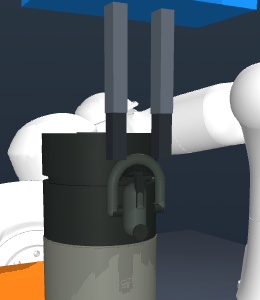
\includegraphics[width=.485\linewidth]{figures/pinch_expert.png}\hfill
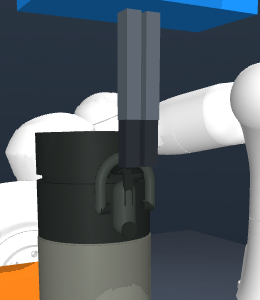
\includegraphics[width=.485\linewidth]{figures/pinch_model_a.png}\\[1pt]
\makebox[.485\linewidth]{\scriptsize expert}\hfill\makebox[.485\linewidth]{\scriptsize model A}
\vspace{6pt}
\end{minipage}
\caption{Left: outcome at every test pose (\ttt{test\_id} and \ttt{test\_ood} together; yaw not shown).
\textcolor{sone}{$\bullet$}~success, \textcolor{stwo}{$\boldsymbol{\times}$}~failure. The dashed square is the
original training box and the solid square the wide box. ACT v2 fails mainly outside its training box. Model A
fails throughout, most often at $y<0$ (3 of 23 \ttt{test\_id} successes there, against 5 of 7 at $y\geq0$).
Right: the pinch at \PinchPose, a \ttt{test\_id} pose. The expert's fingers close on the loop; model A's
fingers close on empty space beside it.}
\label{fig:outcomes}
\end{figure*}

\section{Discussion and limitations}
\begin{itemize}\itemsep0pt
  \item \textbf{Demonstration timing.} This was the largest effect we found: the same model went from \TimedId\%
  to \VtwoId\% by changing when the expert moves on, not what it does. Any scripted or teleoperated data with
  waits that cannot be seen in the observation should be checked for this before training. We showed the
  effect for ACT only. A policy with memory or an explicit phase input might avoid it.
  \item \textbf{Density.} The wide-range results suggest that ACT at this scale (100--300 demonstrations)
  interpolates locally. Extra coverage helps the coarse phases (reaching and folding) but not the precise ones
  (the pinch and the button press) unless the demonstrations are dense near the test poses. More data, longer
  training, or wrist-camera-only inputs for the precise phases are natural next steps.
  \item \textbf{Noise.} Our noise bursts may simply not produce useful recoveries. The noisy collection keeps
  only the 69\% of runs the bursts did not break, so it may contain few real recoveries. Smaller or
  phase-dependent noise, or DAgger~\cite{dagger} with the privileged expert as the teacher, are better-founded
  ways to get recovery data.
  \item \textbf{Statistics.} Each configuration has one training seed, and the test splits are small: 30 and 20
  episodes, with 95\% intervals of $\pm15$--20 points. We ran several comparisons and did not correct for
  that. Only the large effects should be read as established: timed against settle, v2 against A, and A
  against B (with the density caveat). All conclusions hold for this training configuration.
  \item \textbf{Expert baseline.} Our privileged scripted expert fails at yaw below about $-15^\circ$, so the
  wide training data has few demonstrations there. Its 90\% on \ttt{test\_ood} is the score of this scripted
  sequence, not an upper bound on what a policy can reach.
  \item \textbf{Future work.} A longer training run for C would separate undertraining from a coverage and
  precision trade-off. Training on the timed demonstrations with the idle frames down-weighted, or with an
  explicit phase input, would test the idle-wait explanation more directly. Training a diffusion
  policy~\cite{diffusion_policy} or $\pi_0$~\cite{pi0} on both timed and settle demonstrations would show
  whether the timing effect extends beyond ACT.
\end{itemize}

\section{Using the benchmark}
Other policies (e.g.\ a diffusion policy or a fine-tuned VLA such as $\pi_0$~\cite{pi0}) can be compared on
the same footing. Collect settle demonstrations, expose \ttt{make\_policy(pose, **kw)} returning
\ttt{policy(obs, sim)}, then evaluate and print the shared table:
{\scriptsize
\begin{verbatim}
python -m bench.collect --n 100 --settle \
    --out data/expert_v2
python -m bench.evaluate --policy mod:make_policy \
    --split test_id test_ood --name NAME
python -m bench.report
\end{verbatim}}
Use settle demonstrations: ACT trained on timed demonstrations scored 0\% (Sec.~\ref{sec:idle}).

\section{Conclusion}
We turned the detent-bottle environment into a benchmark with randomized poses and fixed held-out splits. We
found that ACT fails on the reference demonstrations, most likely because of idle waits that are not visible
in the observation, and that removing the waits fixes it. An ACT baseline then reaches \VtwoId\% in range and \VtwoOod\% out of range from cameras and
joint readings alone. Widening the training range and adding noise bursts did not reliably improve
out-of-range success with about 200--300 demonstrations. The clearest lesson is that, at this scale,
demonstrations must be dense where the policy is tested.

\paragraph{Acknowledgements.} The environment, bottle mechanism and reference opener are by Jr-Jen Chen. The
\ttt{bench/} code, experiments and this report were produced with the help of Claude Code (Anthropic).

\small\raggedright
\begin{thebibliography}{99}\itemsep0pt
\bibitem{act} T.~Z. Zhao, V.~Kumar, S.~Levine, C.~Finn. Learning fine-grained bimanual manipulation with low-cost hardware. \emph{RSS}, 2023.
\bibitem{dart} M.~Laskey, J.~Lee, R.~Fox, A.~Dragan, K.~Goldberg. DART: Noise injection for robust imitation learning. \emph{CoRL}, 2017.
\bibitem{dagger} S.~Ross, G.~Gordon, D.~Bagnell. A reduction of imitation learning and structured prediction to no-regret online learning. \emph{AISTATS}, 2011.
\bibitem{mujoco} E.~Todorov, T.~Erez, Y.~Tassa. MuJoCo: A physics engine for model-based control. \emph{IROS}, 2012.
\bibitem{gymnasium} M.~Towers et al. Gymnasium: A standard interface for reinforcement learning environments. arXiv:2407.17032, 2024.
\bibitem{resnet} K.~He, X.~Zhang, S.~Ren, J.~Sun. Deep residual learning for image recognition. \emph{CVPR}, 2016.
\bibitem{cvae} K.~Sohn, H.~Lee, X.~Yan. Learning structured output representation using deep conditional generative models. \emph{NeurIPS}, 2015.
\bibitem{rot6d} Y.~Zhou, C.~Barnes, J.~Lu, J.~Yang, H.~Li. On the continuity of rotation representations in neural networks. \emph{CVPR}, 2019.
\bibitem{drq} I.~Kostrikov, D.~Yarats, R.~Fergus. Image augmentation is all you need: Regularizing deep reinforcement learning from pixels. \emph{ICLR}, 2021.
\bibitem{diffusion_policy} C.~Chi, S.~Feng, Y.~Du, Z.~Xu, E.~Cousineau, B.~Burchfiel, S.~Song. Diffusion policy: Visuomotor policy learning via action diffusion. \emph{RSS}, 2023.
\bibitem{pi0} K.~Black et al. $\pi_0$: A vision-language-action flow model for general robot control. arXiv:2410.24164, 2024.
\end{thebibliography}

\end{document}
